\documentclass[a4paper,10pt]{article}
\usepackage[utf8]{inputenc}
\usepackage{amsmath}
\usepackage{graphicx}
\numberwithin{equation}{section}
%opening
\title{Math Phys II HW 2}
\author{Vince Baker}

\begin{document}

\maketitle

\begin{abstract}

\end{abstract}

\section{Problem 1}
We seek solutions of the Kortweg-deVries equation:
\begin{equation}
 \frac{\partial \psi}{\partial t}+\psi\frac{\partial \psi}{\partial x}+\frac{\partial ^3 \psi}{\partial x^3}=0
\end{equation}
We look for solutions $\psi(\xi)$, with $\xi=x-ct$. To write 1.1 in terms of $\xi$, we calculate the partial derivatives:
\begin{gather*}
 \frac{\partial \psi}{\partial t}=-c\frac{d \psi(\xi)}{d \xi}\\
 \frac{\partial \psi}{\partial x}=\frac{d \psi(\xi)}{d \xi}\\
 \frac{\partial^3 \psi}{\partial x^3}=\frac{d^3 \psi(\xi)}{d \xi ^3}
\end{gather*}
We can now write 1.1 in terms of $\xi$:
\begin{equation} 
-c\frac{d \psi}{d \xi}+\psi\frac{d \psi}{d \xi}+\frac{d^3 \psi}{d \xi ^3}=0
\end{equation}
This simplifies to:
\begin{equation}
 (\psi-c)\frac{d \psi}{d \xi}+\frac{d^3 \psi}{d \xi ^3}=0
\end{equation}
We can integrate 1.3 to find:
\begin{equation}
 \frac{d^2\psi}{d\xi^2}=c\psi-\frac{\psi^2}{2}
\end{equation}
We then integrate again and multiply by $\frac{d \psi}{d \xi}$:
\begin{gather}
\frac{d\psi}{d\xi}=\int(c\psi-\frac{\psi^2}{2})\\
(\frac{d\psi}{d\xi})^2=\frac{\psi^2}{2}(c-\frac{\psi}{3})\\
\frac{d\psi}{d\xi}=\frac{\psi}{\sqrt{2}}(c-\frac{\psi}{3})^\frac{1}{2}
\end{gather}
We can now integrate for $\xi$:
\begin{equation}
 d\xi =\int \frac{d \psi}{\frac{\psi}{\sqrt{2}}(c-\frac{\psi}{3})^{\frac{1}{2}}}\\
\end{equation}
And then rearrange to find $\psi$ as a function of $\xi$ and c.

\section{Problem 2}
The general form of a second-order linear PDE is:
\begin{equation}
 A(x,y)\frac{\partial ^2 \psi}{\partial x^2}+2B(x,y)\frac{\partial ^2\psi}{\partial x \partial y}+C(x,y)\frac{\partial ^2 \psi}{\partial y^2}
\end{equation}
The characteristic equation,  with solutions $\xi(x,y)$ and $\eta(x,y)$, is:
\begin{equation}
 A(\frac{dy}{dx})^2+2B(\frac{dy}{dx})+C=0
\end{equation}
We wish to write Eq. 1 in terms of $\xi$ and $\eta$. We differentiate $\psi(\xi, \eta)$:
\begin{gather}
\frac{\partial \psi}{\partial x}=\frac{\partial \psi}{\partial \xi}\frac{\partial \xi}{\partial x}+\frac{\partial \psi}{\partial \eta}\frac{\partial \eta}{\partial x}
\end{gather}
Now we calculate the other partials with respect to $\eta$ and $\xi$.
\begin{gather}
\frac{\partial}{\partial x}(\frac{\partial \psi}{\partial \xi})=\frac{\partial ^2 \psi}{\partial \xi^2}\frac{\partial \xi}{\partial x}+
\frac{\partial ^2 \psi}{\partial \xi \partial \eta}\frac{\partial \eta}{\partial x}\\
\frac{\partial}{\partial x}(\frac{\partial \psi}{\partial \eta})=\frac{\partial ^2 \psi}{\partial \eta^2}\frac{\partial \eta}{\partial x}+
\frac{\partial ^2 \psi}{\partial \xi \partial \eta}\frac{\partial \xi}{\partial x}
\end{gather}
We use 3,4 and 5 to calculate $\frac{\partial ^2 \psi}{\partial x^2}$.
\begin{gather*}
\frac{\partial ^2 \psi}{\partial x^2} = \frac{\partial ^2 \xi}{\partial x^2}\frac{\partial \psi}{\partial \xi}
+\frac{\partial \xi}{\partial x}(\frac{\partial ^2 \psi}{\partial \xi^2}\frac{\partial \xi}{\partial x}+
\frac{\partial ^2 \psi}{\partial \xi \partial \eta}\frac{\partial \eta}{\partial x})\\
+\frac{\partial ^2 \eta}{\partial x^2}\frac{\partial \psi}{\partial \eta}
+\frac{\partial \eta}{\partial x}(\frac{\partial ^2 \psi}{\partial \eta^2}\frac{\partial \eta}{\partial x}+
\frac{\partial ^2 \psi}{\partial \xi \partial \eta}\frac{\partial \xi}{\partial x})\\
=\frac{\partial ^2 \xi}{\partial x^2}\frac{\partial \psi}{\partial \xi}+\frac{\partial ^2 \eta}{\partial x^2}\frac{\partial \psi}{\partial \eta}
+\frac{\partial ^2 \psi}{\partial \xi ^2}(\frac{\partial \xi}{\partial x})^2 +\frac{\partial \xi}{\partial x}\frac{\partial \eta}{\partial x}
\frac{\partial ^2 \psi}{\partial \xi \partial \eta}+\frac{\partial ^2 \psi}{\partial \eta ^2}(\frac{\partial \eta}{\partial x})^2
+\frac{\partial \xi}{\partial x}\frac{\partial \eta}{\partial x}\frac{\partial ^2 \psi}{\partial \xi \partial \eta}
\end{gather*}
\begin{gather}
\frac{\partial ^2 \psi}{\partial x^2}=\frac{\partial ^2 \xi}{\partial x^2}\frac{\partial \psi}{\partial \xi}+\frac{\partial ^2 \eta}{\partial x^2}
\frac{\partial \psi}{\partial \eta}
+\frac{\partial ^2 \psi}{\partial \xi ^2}(\frac{\partial \xi}{\partial x})^2+\frac{\partial ^2 \psi}{\partial \eta ^2}(\frac{\partial \eta}{\partial x})^2
+2(\frac{\partial \xi}{\partial x}\frac{\partial \eta}{\partial x}\frac{\partial ^2 \psi}{\partial \xi \partial \eta})
\end{gather}
The calculation of $\frac{\partial ^2 \psi }{\partial y^2}$ is identical.
\begin{gather}
\frac{\partial ^2 \psi}{\partial y^2}=\frac{\partial ^2 \xi}{\partial y^2}\frac{\partial \psi}{\partial \xi}+\frac{\partial ^2 \eta}{\partial y^2}\frac{\partial \psi}{\partial \eta}
+\frac{\partial ^2 \psi}{\partial \xi ^2}(\frac{\partial \xi}{\partial y})^2+\frac{\partial ^2 \psi}{\partial \eta ^2}(\frac{\partial \eta}{\partial y})^2
+2(\frac{\partial \xi}{\partial y}\frac{\partial \eta}{\partial y}\frac{\partial ^2 \psi}{\partial \xi \partial \eta})
\end{gather}
We now take $\frac{\partial}{\partial y}$ of equation 1:
\begin{multline}
 \frac{\partial ^2\psi}{\partial x \partial y}=\frac{\partial ^2\xi}{\partial x \partial y}\frac{\partial \psi}{\partial \xi}
 +\frac{\partial ^2 \eta}{\partial x \partial y}\frac{\partial \psi}{\partial \eta}
 +\frac{\partial^2 \psi}{\partial \xi ^2}(\frac{\partial \xi}{\partial x}\frac{\partial \xi}{\partial y})\\
 +\frac{\partial^2 \psi}{\partial \eta ^2}(\frac{\partial \eta}{\partial x}\frac{\partial \eta}{\partial y})
 +\frac{\partial ^2 \psi}{\partial \xi \partial \eta}(\frac{\partial \xi}{\partial x}\frac{\partial \eta}{\partial y}+\frac{\partial \eta}{\partial x}\frac{\partial \xi}{\partial y} ) 
\end{multline}

We can now write Eq. 1 in terms of $\xi$ and $\eta$:
\begin{multline}
 A\{\frac{\partial ^2 \xi}{\partial x^2}\frac{\partial \psi}{\partial \xi}+\frac{\partial ^2 \eta}{\partial x^2}
\frac{\partial \psi}{\partial \eta}
+\frac{\partial ^2 \psi}{\partial \xi ^2}(\frac{\partial \xi}{\partial x})^2+\frac{\partial ^2 \psi}{\partial \eta ^2}(\frac{\partial \eta}{\partial x})^2
+2(\frac{\partial \xi}{\partial x}\frac{\partial \eta}{\partial x}\frac{\partial ^2 \psi}{\partial \xi \partial \eta})\}\\
+2B\{\frac{\partial ^2\xi}{\partial x \partial y}\frac{\partial \psi}{\partial \xi}
 +\frac{\partial ^2 \eta}{\partial x \partial y}\frac{\partial \psi}{\partial \eta}
 +\frac{\partial^2 \psi}{\partial \xi ^2}(\frac{\partial \xi}{\partial x}\frac{\partial \xi}{\partial y})\\
 +\frac{\partial^2 \psi}{\partial \eta ^2}(\frac{\partial \eta}{\partial x}\frac{\partial \eta}{\partial y})
 +\frac{\partial ^2 \psi}{\partial \xi \partial \eta}(\frac{\partial \xi}{\partial x}\frac{\partial \eta}{\partial y}+\frac{\partial \eta}{\partial x}\frac{\partial \xi}{\partial y} ) \}\\
 +C\{\frac{\partial ^2 \xi}{\partial y^2}\frac{\partial \psi}{\partial \xi}+\frac{\partial ^2 \eta}{\partial y^2}\frac{\partial \psi}{\partial \eta}
+\frac{\partial ^2 \psi}{\partial \xi ^2}(\frac{\partial \xi}{\partial y})^2+\frac{\partial ^2 \psi}{\partial \eta ^2}(\frac{\partial \eta}{\partial y})^2
+2(\frac{\partial \xi}{\partial y}\frac{\partial \eta}{\partial y}\frac{\partial ^2 \psi}{\partial \xi \partial \eta}) \}
\end{multline}
We now take a break to stop Eq. 9 from giving us a migraine brought on by eye strain.

We collect the coefficients of all the derivates of $\psi$:
\begin{gather*}
\frac{\partial \psi}{\partial \xi}(A\frac{\partial ^2 \xi}{\partial x^2}+2B\frac{\partial ^2 \xi}{\partial x \partial y}+C\frac{\partial ^2 \xi}{\partial y^2})\\
\frac{\partial \psi}{\partial \eta}(A\frac{\partial ^2 \eta}{\partial x^2}+2B\frac{\partial ^2 \eta}{\partial x \partial y}+C\frac{\partial ^2 \eta}{\partial y^2})\\
\frac{\partial ^2 \psi}{\partial \xi ^2}(A(\frac{\partial \xi}{\partial x})^2+2B\frac{\partial \xi}{\partial x}\frac{\partial \xi}{\partial y}+C(\frac{\partial \xi}{\partial y})^2)\\
\frac{\partial ^2 \psi}{\partial \eta ^2}(A(\frac{\partial \eta}{\partial x})^2+2B\frac{\partial \eta}{\partial x}\frac{\partial \eta}{\partial y}+C(\frac{\partial \eta}{\partial y})^2)\\
\frac{\partial ^2 \psi}{\partial \xi \partial \eta}(2A(\frac{\partial \xi}{\partial x}\frac{\partial \eta}{\partial x})
+2B(\frac{\partial \xi}{\partial x}\frac{\partial \eta}{\partial y}+\frac{\partial \xi}{\partial y}\frac{\partial \eta}{\partial y})
+2C(\frac{\partial \xi}{\partial y}\frac{\partial \eta}{\partial x}))
\end{gather*}

After the break, we recognize that since $\xi(x,y)$ and $\eta(x,y)$ are solutions to Eq. 1:
\begin{gather}
 A(\frac{\partial \xi}{\partial x})^2+2B\frac{\partial \xi}{\partial x}\frac{\partial \xi}{ \partial y}+C(\frac{\partial \xi}{\partial y})^2=0\\
 A(\frac{\partial \eta}{\partial x})^2+2B\frac{\partial \eta}{\partial x}\frac{\partial \eta}{ \partial y}+C(\frac{\partial \eta}{\partial y})^2=0
\end{gather}

\section{Problem 3}
We are solving the characteristic equation for:
\begin{gather*}
 \frac{\partial ^2\psi}{\partial t^2}-c(x)^2\frac{\partial ^2 \psi}{\partial x^2}=0\\
\end{gather*}
With A=1, B=0, and $c=-c(x)^2$, the characteristic equation is:
\begin{gather}
(\frac{dx}{dt})^2-c(x)^2=0\\
\frac{dx}{dt}=\pm c(x)\\
dt=\pm\frac{1}{c(x)}dx
\end{gather}
With $c(x)=c_0(1+\frac{|x|}{a})$ the characteristic curve can be written:
\begin{equation}
t=\pm\frac{1}{c_0}(x+sgn(x)\frac{x^2}{2a})+C
\end{equation}
Several characteristic curves are shown below for a-values 0.01, 0.1, 1 and 10. The positive curves are shown in blue, the negative curves in red.

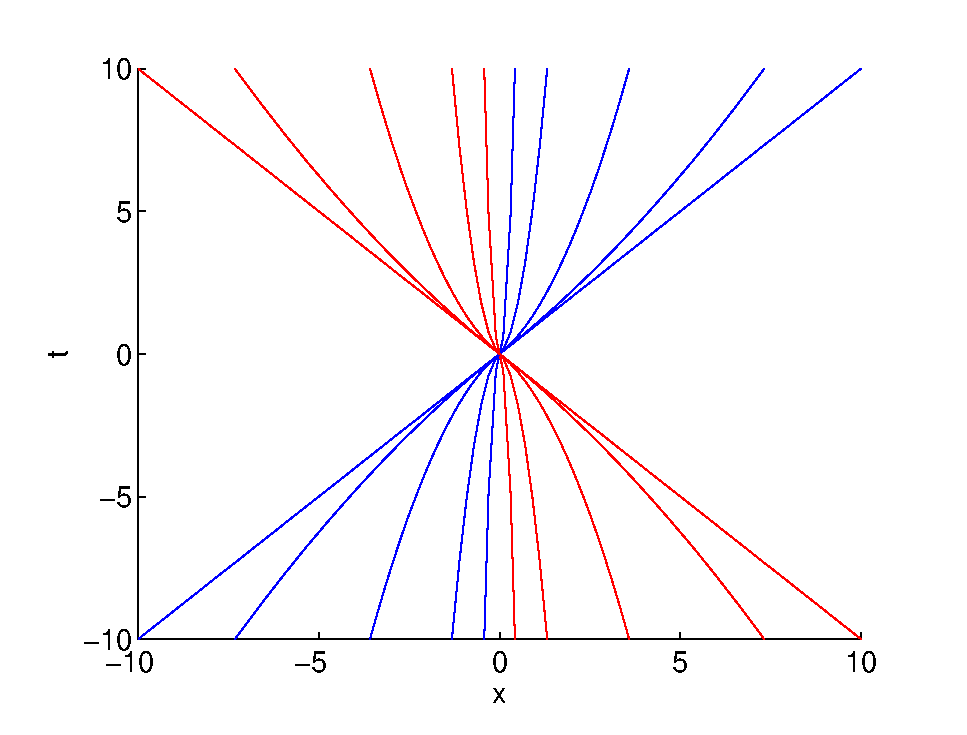
\includegraphics{p3chars}

We now look to find a solution given the initial conditions:
\begin{gather}
\psi(x,0)=0\\
\frac{\partial \psi}{\partial t}\mid_{t=0}=e^{-|x|}
\end{gather}
When $a=\infty$ the characteristic solutions become:
\begin{gather}
\xi=x+c_0t\\
\eta=x-c_0t
\end{gather}
The solution can be written as a combination $\psi=f(\xi)+g(\eta)$. 
Using the initial condition $\psi(x,0)=0$ we see that $f(x)+g(x)=0$, so that $g(x)=-f(x)$.
We differentiate the combined solution with respect to t and use the second boundary condition:
\begin{gather}
-v\frac{df}{dt}+c_0\frac{dg}{dt}=e^{-|x|}\\
\int-2\frac{df}{dt}=\int\frac{1}{c_0}e^{-|x|}\\
f=\frac{-1}{2c_0}e^{-|x|}
\end{gather}
We can now write the combined solution:
\begin{equation}
\psi(x,t)=\frac{1}{2c_0}(e^{-|x+vt|}-e^{-|x-vt|}) 
\end{equation}

\section{Problem 4}
We solve the diffusion equation for the temperature in a uniform cube of side L.

\begin{equation}
 \nabla^2T=\frac{1}{\kappa}\frac{\partial T}{\partial t}
\end{equation}
We first separate T into time and space terms.
\begin{gather}
 T=\Gamma (t)\Psi(\vec{r})\\
 \nabla ^2T=\nabla ^2 \Psi \Gamma\\
 \frac{\partial T}{\partial t}=\Psi \Gamma ^{\prime}\\
 \frac{\nabla ^2 \Psi}{\Psi}-\frac{1}{\kappa}\frac{\Gamma ^{\prime}}{\Gamma}=0\\
 \frac{\nabla ^2 \Psi}{\Psi}=-\frac{1}{\kappa}\frac{\Gamma ^{\prime}}{\Gamma}=-c^2\\
\end{gather}
We can now solve the time dependent part.
\begin{gather}
\Gamma ^{\prime}=\Gamma kc^2\\
\Gamma ^{\prime}-kc^2\Gamma=0\\
\Gamma=\alpha e^{-tkc^2}
\end{gather}
The boundary condition $\Gamma=0$ at $t=0$ can't be satisfied by this equation, so we shift the temperature scale so that the system
starts at $T=-T_0$ and the heat bath is at a temperature of 0. We can then solve for $\alpha$.
\begin{gather}
\alpha = -T_0\\
\Gamma=-T_0 e^{-tkc^2}
\end{gather}

We now separate the X/Y/Z components of the spatial function.
\begin{gather}
\Psi (\vec{r})=X(x)Y(y)Z(z)\\
\frac{\nabla ^2\Psi}{\Psi}=-c^2\\
\nabla ^2\Psi +c^2 \Psi =0\\
X^{''} YZ+XY^{''} Z+XYZ^{''} +c^2XYZ=0\\
\frac{X^{''} }{X}+\frac{Y^{''} }{Y}+\frac{Z^{''} }{Z}+c^2=0\\
X^{''} +\ell^2 X=0\\
Y^{''} +m^2 Y=0\\
Z^{''} +n^2 Z=0\\
\ell ^2+m^2+m^2=-c^2
\end{gather}
The spatial functions are all zero at both 0 and L (since we've shifted the temperature scale so the heat bath is at 0).
The solutions are:
\begin{gather}
X=sin\frac{\alpha \pi}{L}x\\
Y=sin\frac{\beta \pi}{L}y\\
Z=sin\frac{\gamma \pi}{L}z\\
\alpha=\frac{\ell L}{\pi},\ \beta=\frac{mL}{\pi},\ \gamma=\frac{nL}{\pi}
\end{gather}
We can now write the general solution to the equation as a linear combination of the separate solutions.
\begin{equation}
T=\sum _{\alpha,\beta,\gamma=0}^{\infty}\mu_{\alpha \beta \gamma}(-T_0)e^{-tkc^2}\ sin(\frac{\alpha\pi}{L}x)\ sin(\frac{\beta \pi}{L}y)\ sin(\frac{\gamma \pi}{L}z)
\end{equation}
With $\ell, m, n$ integers and subject to $\ell^2+m^2+n^2=-c^2$. We write $c^2$ in terms of $\alpha,\ \beta,\ \gamma$ and pull out the 0th coefficient:
\begin{gather}
c_{\alpha \beta \gamma}^2=\frac{\pi ^2 \alpha ^2}{L^2}+\frac{\pi ^2 \beta ^2}{L^2}+\frac{\pi ^2 \gamma ^2}{L^2}=\frac{\pi ^2}{L ^2}(\alpha ^2+\beta ^2+\gamma ^2)\\
T=-T_0+\sum _{\alpha,\beta,\gamma=0}^{\infty}\alpha_{\alpha \beta \gamma}e^{-tkc_{\alpha \beta \gamma}^2}\ sin(\frac{\alpha\pi}{L}x)\ sin(\frac{\beta \pi}{L}y)\ sin(\frac{\gamma \pi}{L}z)
\end{gather}

\section{Problem 5}
We solve the wave equation for a particle confined to a cylinder of radius R and height H.
\begin{gather}
\frac{-\hbar ^2}{2m} \nabla ^2 \psi=E \psi\\
\nabla ^2 \psi +k^2\psi=0, k\equiv \sqrt{\frac{2mE}{\hbar ^2}}
\end{gather}
We separate the equation into functions in cylindrical coordinates.
\begin{gather}
 \psi=R(r)\Phi(\phi)Z(z)\\
 \frac{1}{r}\frac{\partial}{\partial r}(r\frac{dR}{dr})\Phi Z+\frac{1}{r^2}\frac{d \Phi ^2}{d \phi }RZ+\frac{d^2Z}{dz}R\Phi +k^2r\Phi Z=0\\
 \frac{1}{rR}\frac{d}{dr}(rR^{'} )+\frac{1}{r^2}\frac{\Phi^{''} }{\Phi}+\frac{Z^{''}}{Z}+k^2=0
\end{gather}
We can now solve for Z incorporating the boundary conditions that $\psi=0$ at z=0,H.
\begin{gather}
\frac{Z^{''}}{Z}=const.=\ell ^2\\
 Z^{''}-\ell ^2Z=0\\
 Z=sin\frac{\ell \pi}{H}z
\end{gather}
Substituing the constant value of $\frac{Z^{''}}{Z}$ into 5.5 and multiplying by $r^2$, we get:
\begin{equation}
\frac{r}{R}\frac{d}{dr}(rR^{'})+\frac{\Phi ^{''}}{\Phi}+r^2(\ell ^2+k^2)=0 
\end{equation}
we can now separate the $\Phi$ term.
\begin{gather}
\frac{\Phi ^{''}}{\Phi}=const.=-m^2\\
\Phi ^{''}+m^2\Phi=0
\end{gather}
There is no explicit boundary condition on $\phi$. 
However, since $\phi$ is an angular coordinate $\Phi$ must be single-valued on multiples of $2\pi$. 
With $\Phi(0)=\Phi(2\pi)$, the solution is a general exponential with m confined to integer values.
\begin{equation}
\Phi=e^{im \phi}, \  m=0,1,2...
\end{equation}

\end{document}
